\documentclass[xcolor=dvipsnames]{beamer}
\usepackage[orientation=landscape,size=a0,scale=1.,debug]{packages/beamerposter}
\usepackage{wasysym}
\usepackage{eurosym}
\usepackage{ulem}
\usepackage{soul}
\usepackage{pifont}
\usepackage{graphicx}
\usepackage{multirow}
\usepackage{shadow}
\usepackage{tikz}
\usepackage{eso-pic,rotating} 
\usepackage[mathbf,mathcal,text-hat-accent]{euler} 
\usepackage{amsmath} 
\usepackage{xcolor}
\usepackage{enumitem}
\usepackage{enumerate}
\usepackage{overpic}
\usepackage[export]{adjustbox}
\usepackage{ragged2e}
\usepackage[french]{babel}
\usepackage[utf8x]{inputenc}
\usepackage[T1]{fontenc}
\usepackage[most]{tcolorbox}


% \usefonttheme[onlymath]{serif}

\usetikzlibrary{arrows,positioning,shapes}
\usetikzlibrary{tikzmark,positioning}

\setbeamertemplate{items}[triangle]

%%%%%%%%%%%%%%%%%%%% 

\newcommand{\thetitleter}{CHyMENE}
\newcommand{\thetitlebis}{EBRAINS Neuromorphic Computing}
\newcommand{\thepurpose}{INCF Assembly 2021}
\newcommand{\thedate}{N 19th, 2021}
\newcommand{\thetitle}{Providing community access to large-scale neuromorphic computing systems}
\newcommand{\theauthor}{Matthieu Sénoville}
\newcommand{\theauthorbis}{Matthieu Sénoville, on behalf of EBRAINS Neuromorphic Computing Collaboration}
\newcommand{\theauthorlist}{\underline{\textbf{M.~S\'{e}noville}}$^{1}$, H. Aguili$^{1}$, O. Ate\c{s}$^{1}$, J. Duperrier$^{1}$, D. Guarino$^{1}$, B. Lungsi Sharma$^{1}$, E. Müller$^{2}$, A.G.D. Rowley$^{3}$, A.P. Davison$^{1}$\\[3mm] and the EBRAINS Neuromorphic Computing Collaboration}
\newcommand{\theaffiliations}{  $^{1}$Paris-Saclay Institute of Neuroscience, UMR 9197, Centre National de la Recherche Scientifique/Université Paris-Saclay, France\\
                                $^{2}$Kirchhoff Institute for Physics, Heidelberg University, Heidelberg, Germany\\
                                $^{3}$Advanced Processor Technologies Group, Department of Computer Science, University of Manchester, Manchester, United Kingdom}
\newcommand{\theemail}{matthieu.senoville@cnrs.fr}
\newcommand{\thelabo}{Paris-Saclay Institute of Neuroscience}
\newcommand{\reducedlabo}{NeuroPSI}
\newcommand{\urllabo}{https://ebrains.eu/service/neuromorphic-computing/}

%%%%%%%%%%%%%%%%%%%% 

\title{\Huge{\textbf{\thetitle}}}
\author{\textbf{\Large{\theauthor}}}
\institute{\large{\thelabo}}

% \setbeamertemplate{headline}{  
%     \begin{tikzpicture}[remember picture,overlay,thick]
%       \node[draw=none,fill=none] at (\paperwidth*0.5,10cm) {
\includegraphics[trim=0 23 0 90, clip, width=150cm]{/home/matthieu/Documents/HBP/SP9/logos/HBP_pure.pdf}};
%     % \shade [left color=black,right color= red]
%     % \useasboundingbox (0,0) rectangle (\paperwidth, -10cm);
%     % 
\includegraphics[width=\paperwidth]{/home/matthieu/Documents/HBP/SP9/logos/HBP_pure.pdf}
%     % \pgftext[at=\pgfpoint{0cm}{0cm}, left, base]{\pgfuseimage{/home/matthieu/Documents/HBP/SP9/logos/HBP_pure.pdf}}; 
%     \end{tikzpicture}
%     \vskip2.cm
% \begin{center}
% \usebeamercolor{title in headline}{\color{black}\textbf{\VERYHuge{\inserttitle}}\\[1ex]}
% \vskip0.8cm
%  			\center{
      
%             \usebeamercolor{author in headline}{\color{black}\normalsize{\textbf{\underline{M. Sénoville}, 
%             O. Ate\c{s},
%             J. Duperrier,
%             D. Guarino,
%             A.P. Davison
%             }}}}
%             \vskip0.9cm
%             \usebeamercolor{institute in headline}{\color{black}
%                 \center{\large{\textbf{Unité de Neurosciences, Information et Complexité, CNRS, Gif-sur-Yvette, France}}\\[11mm]
%                 \normalsize{\textbf{and the HBP-SP9 Neuromorphic Computing Collaboration}}}
%             }

%      \end{center}
% %     \vskip0.3cm
% %   \end{beamercolorbox}
%  }

% \setbeamertemplate{footline}{
%   \begin{flushright}
%     \begin{minipage}{1.0\linewidth}
%       % here, you can add some other logos
%       \hfill \hfill
%       %\includegraphics[width=8.7cm]{\packpath/logolpc.pdf}
%       \vspace{+2.mm} %\includegraphics[height=4cm]{\imgpath/HBPLogo.png} 
%       % \includegraphics[height=3.0cm]{\imgpath/HBP.png} \quad
%       
\includegraphics[height=2cm]{\imgpath/FraunhoferLOGO_0.jpg} \quad
%       
\includegraphics[height=2cm]{\imgpath/TU_Dresden.jpg} \quad
%       
\includegraphics[height=2cm]{\imgpath/CNRS.png}\quad      
%       
\includegraphics[height=2cm]{\imgpath/TU_Graz.png}  \quad
%       \includegraphics[height=2cm]{\imgpath/university-of-hertfordshire2.png} \quad
%       
\includegraphics[height=2cm]{\imgpath/Heidelberg.png} \quad     
%       
\includegraphics[height=2cm]{\imgpath/istanbul.png} \quad
%       
\includegraphics[height=2cm]{\imgpath/Logo_EPFL.png} \quad
%       
\includegraphics[height=2cm]{\imgpath/middlesex.png}\quad
%       
\includegraphics[height=2cm]{\imgpath/manchester.png} \quad
%       
\includegraphics[height=2cm]{\imgpath/Kth_logo.png} \quad
%       
\includegraphics[height=2cm]{\imgpath/turin.jpeg} \quad     
%       
\includegraphics[height=2.8cm]{\imgpath/eu_cofunded_logo.png}
%     \end{minipage}
%   \end{flushright}
%   \vspace{-42mm}  
%   \begin{flushleft}
%       \includegraphics[height=3.2cm]{\imgpath/HBP.png} \quad
%   \end{flushleft}   
%   \begin{beamercolorbox}[ht=2\baselineskip,leftskip=0.9cm,rightskip=0.6cm]{footline}
%     \vspace{-4mm}
%     \begin{small}\textbf{\theauthorbis} \end{small} \hfill \hfill
%     \begin{small}\texttt{\textbf{\theemail}} \end{small} \hfill \hfill
%     % \begin{small}\texttt{\textbf{\theemail}} \qquad and \qquad \texttt{\textbf{other email}}\end{small} \hfill \hfill
%     \begin{small}\textbf{\urllabo} \end{small}
%     \vspace{0.5cm}
%   \end{beamercolorbox}
%   \begin{beamercolorbox}[wd=\paperwidth]{lower separation line foot}
%     \rule{0pt}{2pt}
%   \end{beamercolorbox}
% }


% \newcommand{\thelineHBP}{
% 	\setbeamercolor*{block body}{bg=white,fg=white}
% 	\setbeamercolor*{block title}{fg=BurntOrange,bg=BurntOrange}
% 		\begin{tikzpicture}[remember picture,overlay,thick]
% 		\node[draw=none,fill=none] at (\paperwidth*0.5-1cm,0cm) {\includegraphics[trim=0 19 0 141., clip, width=150cm]{\imgpath/HBPlogo.png}};
% 		\end{tikzpicture}
% 	\setbeamercolor*{block body}{bg=lgray,fg=black}
% 	\setbeamercolor*{block title}{fg=black,bg=sp9}
% }
\newtcolorbox{myblock22}[2][]{
    % empty,
    % beamer,
    title=#2,fonttitle=\sffamily,
  left=0mm,right=0mm,top=0mm,bottom=0mm,arc=0mm,
%   height fill,
  colback=white, colbacklower=white, colupper=black, colframe=green,
  coltitle=black,title style={left color=green!70, right color=green!20},
%   colback={top color=white, bottom color=black},
%   opacityframe=0.25,
  #1}

\newtcolorbox{myblock1}[2][]{
  beamer,
  width=\textwidth-3pt,
  enlarge left by=-0pt,
  colback=structure,
  colframe=white,
  bottom=0pt,
  top=-2pt,
  left=0pt,
  right=0pt,
  toptitle=-1pt,
  bottomtitle=-1pt,
%   fonttitle=\normalfont,
%   adjusted title=#2,
    title=\hskip8mm #2,
    coltitle=black,
  interior titled code={
    \shade[left color=ebrains1!80,right color=ebrains2!80]
    % ,middle color=Salmon] 
      (title.south west) --
      (title.south east) {[rounded corners] -- 
      (title.north east)  -- 
      (title.north west)} --
      (title.south west); 
  }
}

\newtcolorbox{myblock2}[2][]{
  beamer,
  width=\textwidth-3pt,
  enlarge left by=-0pt,
  colback=structure,
  colframe=white,
  bottom=0pt,
  top=-2pt,
  left=0pt,
  right=0pt,
  toptitle=-1pt,
  bottomtitle=-1pt,
%   fonttitle=\normalfont,
%   adjusted title=#2,
    title=\hskip8mm #2,
    coltitle=black,
  interior titled code={
    \shade[left color=ebrains2!80,right color=ebrains3!80]
    % ,middle color=Salmon] 
      (title.south west) --
      (title.south east) {[rounded corners] -- 
      (title.north east)  -- 
      (title.north west)} --
      (title.south west); 
  }
}

\newcommand{\myitem}{$\bullet$}
\newdimen\ratio
\ratio=0.4mm
\newdimen\x
\x=0.3mm

\usecolortheme{default}
\useinnertheme{rounded}

\newcommand{\headlineintro}{
    \vskip22mm
	\center{
		\usebeamerfont*{frametitle}\textbf{\color{black}\VERYHuge{\textbf{\thetitle}}\\[8mm]}
        % \fontsize{100}{120}\selectfont
        % \usebeamerfont*{frametitle}\textbf{\color{black}\textbf{\thetitle}\\[8mm]}
		{\color{black}\normalsize{\textbf{\theauthorlist}}}\\[4mm]
		{\color{black}\footnotesize{\textbf{\theaffiliations}}}
	}
	\vskip16.mm %ou 10 si vert
	\centering
    \begin{tikzpicture}[remember picture,overlay,thick]
        \node[draw=none,fill=none] at (\paperwidth*0.5,4mm) {\adjincludegraphics[trim=0 29.8 0 130.1, clip, width=1.5\paperwidth, cfbox=black 0.pt 0pt 0pt]{\imgpath/HBP_pure.png}};
		% \node[draw=none,fill=none] at (\paperwidth*0.5,4mm) {\adjincludegraphics[trim=0 30 0 130.1, clip, width=1.5\paperwidth, cfbox=black 0.1pt 0pt 0pt]{\imgpath/HBP_pure.pdf}};
	\end{tikzpicture}
	% \begin{tikzpicture}[remember picture,overlay,thick]
	% 	\node[draw=none,fill=none] at (\paperwidth*0.5-0.07cm,0cm) {
\includegraphics[trim=0 50 0 189.5, clip, width=1.35\paperwidth]{\imgpath/EBRAINS_circle.pdf}};
	% \end{tikzpicture}
}


% \newcommand{\headlineframetitle}{

% 	\begin{columns}[t]
% 		\column{0.2\paperwidth} 
% 			\hskip1.mm \vskip1.mm
% 			\includegraphics[trim=0 0 0 0, clip, width=2cm]{\imgpath/EBRAINS_all2.pdf} 
% 		\column{0.7\paperwidth}
% 			\begin{flushright}
% 				\usebeamerfont*{frametitle}\textbf{
% 					\insertframetitle
% 				}
% 			\end{flushright}
% 	\end{columns}	

% 	\vskip1.mm
% 	\centering
% 	\begin{tikzpicture}[remember picture,overlay,thick]
% 		\node[draw=none,fill=none] at (\paperwidth*0.5-0.07cm,0cm) {
\includegraphics[trim=0 50 0 189.5, clip, width=1.35\paperwidth]{\imgpath/EBRAINS_circle.pdf}};
% 	\end{tikzpicture}
% 	\hskip-1mm

% }

% \newcommand{\headlineframetitlebis}{
% 	%   \leavevmode%
% 	%   \hbox{%
% 	%   \begin{beamercolorbox}[wd=\paperwidth,ht=8.25ex,dp=3.5ex]{headertitle}%
% 	% 	% \begin{tikzpicture}[remember picture,overlay,thick]
% 	% 	% 	\node[draw=none,fill=none] at (\paperwidth*0.0-0.00cm,0cm) {\includegraphics[trim=0 0 0 0, clip, width=4cm]{\imgpath/EBRAINS_all.pdf}};
% 	% 	% \end{tikzpicture}
% 	% 	% \hspace*{2em}%
% 		% \Large\color{black}\thetitle %
% 	% 	\begin{center}
% 	%   %   \usebeamercolor{title in headline}{\color{black}\normalsize{\textbf{\thetitle}}\\}
% 	% %   \vskip0.8cm
% 	% 		\insertframetitle
% 	% 			\end{center}
% 	% 	% \hspace*{2em}%
% 	% 	\end{beamercolorbox}%
% 	\begin{columns}[t]
% 		\column{0.2\paperwidth} 
% 		\hskip1.mm \vskip1.mm
% 		\includegraphics[trim=0 0 0 0, clip, width=2cm]{\imgpath/EBRAINS_all2.pdf} 
% 		% \begin{beamercolorbox}[wd=0.8\paperwidth,ht=3.2ex,dp=0ex,left]{frametitle}
% 			% \begin{tikzpicture}[remember picture,overlay,thick]
% 			% \shade [left color=sp9,right color= sp9]
% 			% (-2,-0.262) rectangle (.915\paperwidth,3.2ex);
			
% 			\column{0.7\paperwidth}
% 			% \end{tikzpicture}
% 			\begin{flushright}
% 				\usebeamerfont*{frametitle}\textbf{
% 					\insertframetitle
% 					}
% 			\end{flushright}
% 		\end{columns}	

% 			%   \end{beamercolorbox}
% 		% \begin{beamercolorbox}[wd=0.90\paperwidth,ht=3.2ex,dp=0ex,left]{frametitle}
% 			% \insertframetitle
% 			% \usebeamerfont*{frametitle}\textbf{\frametitle}
% 		% \end{beamercolorbox}\\
% 		% \hfill 
% 		% \insertframetitle
% 		\vskip1.mm
% 		\centering
% 		\begin{tikzpicture}[remember picture,overlay,thick]
% 			\node[draw=none,fill=none] at (\paperwidth*0.5-0.07cm,0cm) {
\includegraphics[trim=0 50 0 189.5, clip, width=1.35\paperwidth]{\imgpath/EBRAINS_circle.pdf}};
% 		\end{tikzpicture}
% 		\hskip-1mm
% 	  }


% \setbeamertemplate{frametitle}{

% }

% \newcommand{\footlineframe}{ 
% % \setbeamertemplate{footline}{
% 	\leavevmode
% 			\vskip-3mm
% 			\begin{tikzpicture}[remember picture,overlay,thick]
% 				% \node[draw=none,fill=none] at (\paperwidth*0.5,4mm) {\includegraphics[trim=0 560 0 1093, clip, width=1.5\paperwidth]{\imgpath/HBPLogo.png}};
% 				\node[draw=none,fill=none] at (\paperwidth*0.5,4mm) {\adjincludegraphics[trim={0 30 0 130.1}, clip, width=1.5\paperwidth, cfbox=black .10pt 0pt 0pt]{\imgpath/HBP_pure.pdf}};
% 			\end{tikzpicture}
% 				
\includegraphics[trim=0 0 0 0, clip, width=0.11\paperwidth]{\imgpath/HBP_large.png} 
% 			\begin{beamercolorbox}[wd=.70\paperwidth,center]{footline1}
% 				\begin{tikzpicture}[remember picture,overlay,thick]
% 				\node[draw=none,fill=none] at (0,1.5mm) {		
% 					\textcolor{DarkSlateGray4}{
% 						\centering \thepurpose \hspace{2cm} \theemail \hspace{2cm} \insertframenumber{} / \inserttotalframenumber \hfill 
% 			   		}
% 			   };
% 			\end{tikzpicture}	
% 		\end{beamercolorbox}
% 		\hfill 
\includegraphics[trim=0 0 0 0, clip, width=0.09\paperwidth]{\imgpath/eu_cofunded_logo.png}

% }

\newcommand{\footlinetitleslide}{
	% \leavevmode
    \vskip-4cm
	\begin{tikzpicture}[remember picture,overlay,thick]
        \node[draw=none,fill=none] at (\paperwidth*0.5,4mm) {\adjincludegraphics[trim=0 29.8 0 130.1, clip, width=1.5\paperwidth, cfbox=black 0.pt 0pt 0pt]{\imgpath/HBP_pure.png}};
		% \node[draw=none,fill=none] at (\paperwidth*0.5,4mm) {\adjincludegraphics[trim=0 30 0 130.1, clip, width=1.5\paperwidth, cfbox=black 0.1pt 0pt 0pt]{\imgpath/HBP_pure.pdf}};
	\end{tikzpicture}
	\vskip-3.0mm
    \phantom{$-$}\\
    % \phantom{-}\\
    % \phantom{-}\\
    % \phantom{-}\\
	
\includegraphics[width=0.12\paperwidth]{\imgpath/HBP_large.png} \quad 
	
\includegraphics[height=23mm]{\imgpath/FraunhoferLOGO_0.jpg} \quad
	
\includegraphics[height=23mm]{\imgpath/logo_bern_uncroped.png} \quad
	
\includegraphics[height=23mm]{\imgpath/citec-uni.jpg} \quad
	
\includegraphics[height=23mm]{\imgpath/TU_Dresden.jpg} \quad
	
\includegraphics[height=23mm]{\imgpath/CNRS.png}\quad      
	
\includegraphics[height=23mm]{\imgpath/TU_Graz.png}  \quad
	
\includegraphics[height=23mm]{\imgpath/university-of-hertfordshire.png} \quad
	
\includegraphics[height=23mm]{\imgpath/Heidelberg.png} \quad     
	
\includegraphics[height=23mm]{\imgpath/istanbul.png} \quad
	
\includegraphics[height=23mm]{\imgpath/Logo_EPFL.png} \quad
	
\includegraphics[height=23mm]{\imgpath/middlesex.png}\quad
	
\includegraphics[height=23mm]{\imgpath/manchester.png} \quad
	
\includegraphics[height=23mm]{\imgpath/Kth_logo.png} \quad
	
\includegraphics[height=23mm]{\imgpath/unisussex.png} \quad
	
\includegraphics[height=23mm]{\imgpath/turin.jpeg} \quad
	
\includegraphics[width=0.09\paperwidth]{\imgpath/eu_cofunded_logo.png}
    \begin{columns}[t]
        \centering
        \column{0.820\textwidth}
        \column{0.16\textwidth}
        \vskip-24mm
        \scriptsize
        This research has received funding from the European Union’s Horizon 2020 Framework Programme for Research
         and Innovation under the Specific Grant Agreement No. 945539 (HBP SGA3), 785907 (HBP SGA2), 
         720270 (HBP SGA1) and the FP7 grant number 604102 (HBP RUP).
    \end{columns}
}


%%%%%%%%%%%%%%%%%%%% 

\begin{document}
\setbeamertemplate{background}{}
\setbeamertemplate{headline}{\headlineintro}
\setbeamertemplate{footline}{\footlinetitleslide}
    \begin{frame}{}
        \vskip52mm
        \begin{columns}[t]
            \centering
            \column{0.40\textwidth}
                \begin{myblock1}{\Large The EBRAINS Neuromorphic Computing Platform \phantom{\Huge $\beta$}}

    \begin{tikzpicture}[remember picture,overlay]
        \node[xshift=-560mm,yshift=265mm] at (current page.center) {
            \adjincludegraphics[trim={0 {.0\height} 0 {.0\height}}, clip, width=30mm, cfbox=black 0.0pt 0pt 0pt]{\imgpath/EBRAINS_circle_2.pdf}
        };
    \end{tikzpicture}

    \vskip13mm
    % \large
    \centering{
        \textbf{EBRAINS} Research Infrastructure offers access to two unique large-scale neuromorphic computing systems:
    }

    \vskip6mm
    \begin{columns}[t]
        \begin{column}{0.46\textwidth}
            \begin{flushright}
                \underline{\textbf{BrainScaleS} : the physical model machine}\\[1mm]
                \scriptsize{Location: Heidelberg (Germany)}
            \end{flushright}
            \vskip-8mm
            \begin{columns}[c]
                \begin{column}{0.50\textwidth}
                    \vskip+3mm
                    \begin{figure}[t]
                        \centering
                        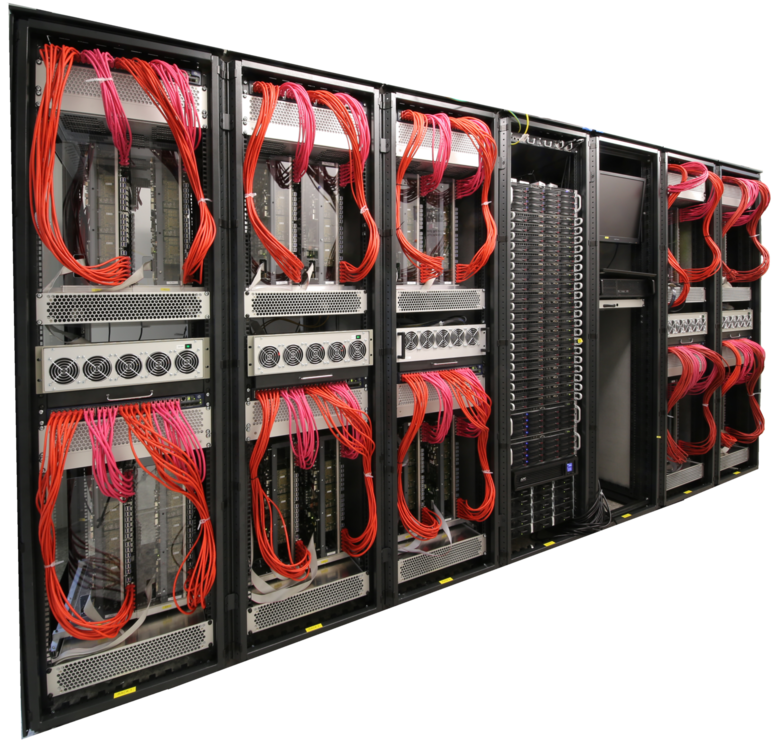
\includegraphics[width=1.0\textwidth,angle=00]{\imgpath/SP9_UHEI_RollUp_20160331_PlatformExported.png}
                    \end{figure}
                \end{column}
                \begin{column}{0.50\textwidth}
                    \begin{flushright}
                        \small{
                            20 wafer modules\\[2mm]

                            Local analogue computing\\
                            4 million neurons \\
                            1 billion plastic synapses\\[2mm]

                            Binary, asynchronous communication\\[2mm]

                            running at x10000 real-time
                        }
                    \end{flushright}
                \end{column}
            \end{columns}
        \end{column}
        % \begin{column}{0.001\textwidth}

        % \end{column}
        \begin{column}{0.46\textwidth}
            \begin{flushleft}
                \underline{\textbf{SpiNNaker} : the many-core machine}\\[1mm]
                \scriptsize{Location: Manchester (UK)}
            \end{flushleft}
            \vskip-9mm
            \begin{columns}[c]
                \begin{column}{0.40\textwidth}
                    \begin{flushleft}
                        \small{
                            over 1 million cores\\[2mm]

                            up to 1 billion neurons \\
                            up to 1 trillion synapses\\[2mm]

                            address-based, small packet, asynchronous communication\\[2mm]

                            real-time simulation
                        }
                    \end{flushleft}
                \end{column}
                \begin{column}{0.60\textwidth}
                    \vskip+3mm
                    \begin{figure}[t]
                        \centering
                        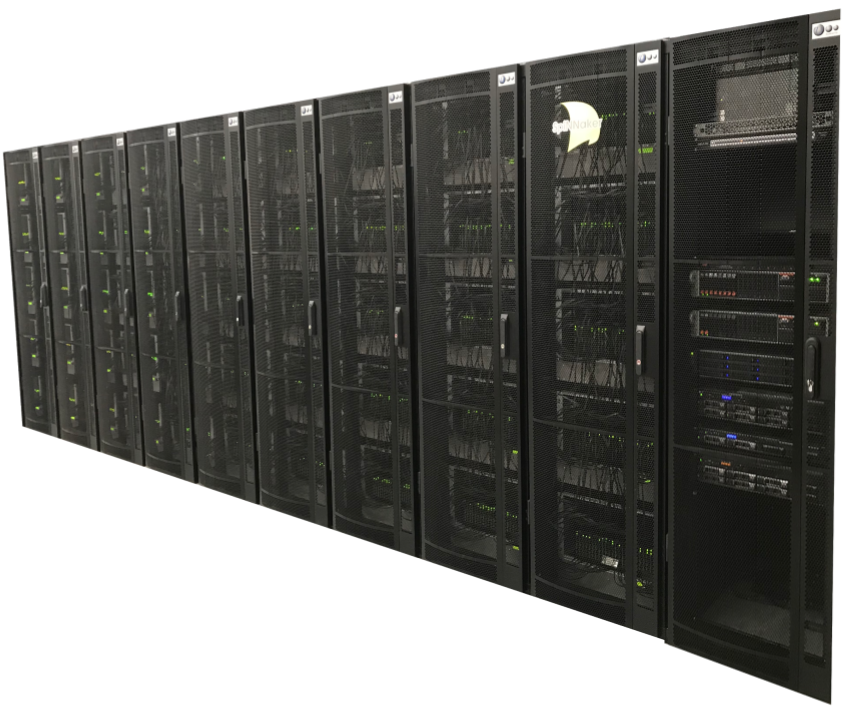
\includegraphics[width=.95\textwidth,angle=00]{\imgpath/SpNN_1Million.png}
                    \end{figure}
                \end{column}
            \end{columns}
        \end{column}
    \end{columns}
    \vskip-15mm
    \begin{columns}[t]
        \begin{column}{0.46\textwidth}
            \hspace{55mm} 
\includegraphics[height=27mm]{\imgpath/BrainScalesLogoNew}
        \end{column}
        % \begin{column}{0.03\textwidth}

        % \end{column}
        \begin{column}{0.46\textwidth}
            \hspace{80mm} 
\includegraphics[height=39mm]{\imgpath/SpiNNlogoHiResGIMP.png}
        \end{column}
    \end{columns}
\end{myblock1}
                \vskip-15mm
                \newcommand{\simulator}{simulator}

\begin{myblock1}{\Large PyNN : a common API for neuronal network modelling \phantom{\Huge $\beta$}}
    
	\vskip-10mm
	\begin{columns}[c]
		\column{.50\textwidth}
		\uncover<1->{
			\hspace{-8mm}
			\begin{itemize}
				\item[$\rhd$] facilitate model sharing and reuse
				\item[$\rhd$] simplify validation of simulation results
				\item[$\rhd$] provide a common platform on which to build other tools
				\item[$\rhd$] provide a more powerful API for neuronal network modelling
				\item[$\rhd$] hide complexity of parallelization from user
			\end{itemize}
		}
		\column{.45\textwidth} 
		\vskip30mm
		\only<1>{\includegraphics[width=0.99\textwidth,angle=00]{\imgpath/pynn.pdf}}
	\end{columns}
	\vspace{5mm}
	
	\begin{columns}[c]
		\column{.50\textwidth}
		\footnotesize
		\only<1>{\texttt{\textcolor{red}{import pyNN.nest as \simulator}}\newline}
		\only<1>{\texttt{\textcolor{red}{import pyNN.neuron as \simulator}}\newline}
		\only<1>{\texttt{\textcolor{red}{import pyNN.brian as \simulator}}\newline}
		\only<1>{\texttt{\textcolor{red}{import pyNN.brainscales as \simulator}}\newline}
		\only<1->{\texttt{\textcolor{red}{import pyNN.spiNNaker as \simulator}}\newline}
		            
		\texttt{cell\_type = \dots}\newline
		
		\only<1->{\texttt{p1 = \textcolor{red}{\simulator}.\textbf{Population(}size1, cell\_type, structure\textbf{)}}}\newline
		\only<1->{\texttt{p2 = \textcolor{red}{\simulator}.\textbf{Population(}size2, another\_cell\_type, structure\textbf{)}}}\newline
		            
		\only<1->{\texttt{all = p1 + p2}}\newline
		\only<1->{\texttt{all.record(["spikes", "v"])}}\newline
		            
		\only<1->{\texttt{connections = \textcolor{red}{\simulator}.\textbf{Projection(}p1, p2, connection\_rule, synapse\_type\textbf{)}}}\newline
		   
		\texttt{\textcolor{red}{\simulator}.run(1000.)}\newline
		            
		\column{.45\textwidth} 
		\vskip+6mm
		\normalsize
		% \fontsize{6}{9}\selectfont
		PyNN is a \textbf{simulator-independent language} for building spiking neuronal network models and provides a library of:
		\begin{itemize}
			\item$\rhd$ standard neuron, synapse and synaptic plasticity models
			\item$\rhd$ commonly-used connectivity algorithms \\[4mm]
		\end{itemize}
		The user is not restricted to the standard models and can also use any neuron or synapse model supported by your simulator.\\[24pt]
		            
		For downloads and full documentation see:\\[4pt]
		\centering{\texttt{\textbf{http://neuralensemble.org/PyNN/}}}
		\normalsize
		
	\end{columns}

\end{myblock1}
                \vskip-15mm
                \begin{myblock1}[noframenumbering]
    \frametitle{}

    \begin{columns}[c]

        \column{0.45\textwidth}
        \begin{figure}
            \centering                
            \includegraphics[height=16cm]{\imgpath/qrcode.png}\\
            \small{\texttt{\textbf{https://ebrains.eu/service/neuromorphic-computing/}}}
        \end{figure}
        \vspace{-5mm}
        \phantom{-}
   

        \column{0.55\textwidth}
            \textbf{\LARGE Request free test access \normalsize} \\[9mm]                      

            \begin{Large}
                \begin{itemize}
                    \item[$\triangleright$] To receive support and advice, visit \\[2mm] 
                    \item[] \texttt{\textbf{https://ebrains.eu/support/}}
                \end{itemize}                   
            \end{Large}
     
      
    \end{columns}

\end{myblock1}

            \column{0.60\textwidth}
                \newlength{\shiftx}
\newlength{\shifty}
\setlength{\shiftx}{-500mm}
\setlength{\shifty}{11.1mm}

\begin{myblock2}{\Large Access through the Collaboratory \phantom{\Huge $\beta$}}
	
	% \vspace{+5.cm}
	% \vspace{-23.8mm}\hspace{+25mm}\tikzmark{ptd}
	% \vspace{+23.8mm}\hspace{-25mm}
	% \vspace{-39.8mm}\hspace{+91mm}\tikzmark{ptf}
	% \vspace{+39.8mm}\hspace{-91mm}
	% \vspace{-.3cm}
	
	\begin{figure}[t]
		\centering
		\adjincludegraphics[trim={0 {.02\height} 0 {.00\height}}, clip, width=1.0\textwidth]{\imgpath/picture-collab-neutre}
		% \includegraphics[width=1.\textwidth,angle=00]{\imgpath/picture-collab-neutre}
	\end{figure}
	\vspace{-130mm}
	\begin{columns}[t]
		\column{.24\textwidth}
		            
		\column{.35\textwidth}
		\begin{normalsize}
			\justify
			\setlength{\parindent}{0mm} 
			The Neuromorphic Job Manager is a web based app providing a graphical interface for submitting jobs
			to the BrainScaleS and SpiNNaker systems and for retrieving job results,
			with detailed provenance metadata including full log files.\\[2mm]
			\justify 
			As a Community app the Job Manager is integrated into the EBRAINS Collaboratory, which aims to be a workspace for scientific collaboration,
			sharing and collaboration around data, software and services.    
			\\[24mm]
			\phantom{-}
		\end{normalsize}
		\column{.3\textwidth}
		
	\end{columns}
	    
	% \begin{tikzpicture}[remember picture,overlay]
	% 	\node[xshift=\shiftx+0cm,yshift=\shifty+0cm] at (current page.center) {
	% 		\adjincludegraphics[trim={0 {.20\height} 0 {.00\height}}, clip, width=0.6\textwidth, cfbox=black 0.1pt 0pt 0pt]{\imgpath/screenshot/collab/fichier-57.png}
	% 	};
	% \end{tikzpicture}
	% \begin{tikzpicture}[remember picture,overlay]
	% 	\node[xshift=\shiftx+45mm,yshift=\shifty+-0.06\textheight] at (current page.center) {
	% 		\adjincludegraphics[trim={0 {.2\height} 0 {.00\height}}, clip, width=0.3*25cm, cfbox=white 0.0pt 0pt 0pt]{\imgpath/screenshot/list/fichier-3-wo-space.png}
	% 	};
	% \end{tikzpicture}
	% \begin{tikzpicture}[remember picture,overlay,
	% 	arrow/.style={red!80!black,thin,->,>=latex,outer sep=-.5cm}]
	% 	\node[xshift=0.373\textwidth,yshift=-0.024\textheight](jobcreation) at (current page.center) {
	% 		\adjincludegraphics[trim={0 0 0 {.004\height}}, clip, width=0.3\textwidth, cfbox=red!80!black 0.1pt 0pt -2.5pt]{\imgpath/screenshot/create/fichier-30.png}
	% 	};
	% 	\draw[arrow]
	% 	(jobcreation) to[out=180,in=0] ([yshift=6.7mm]{pic cs:ptf}); 
	% \end{tikzpicture}
	% \begin{tikzpicture}[remember picture,overlay,
	% 	arrow/.style={red!80!black,thin,->,>=latex,outer sep=-.5cm}]
	% 	\node[xshift=-0.4\textwidth,yshift=-0.19\textheight](jobdetails) at (current page.center) {
	% 		\adjincludegraphics[trim={0 {.3\height} 0 {.000\height}}, clip, width=0.25\textwidth, cfbox=red!80!black 0.1pt 0pt -2.5pt]{\imgpath/screenshot/details/fichier-9.png}
	% 	};
	% 	\draw[arrow]
	% 	(jobdetails) to[out=90,in=180] ([yshift=-0.mm]{pic cs:ptd}); 
	% \end{tikzpicture}
	
\end{myblock2}
                \vskip-15mm
                \definecolor{pyblue}{RGB}{11, 87, 168}
\definecolor{pygreen}{RGB}{15, 127, 18}
\definecolor{pyred}{RGB}{184, 35, 39}
\definecolor{pyjup}{RGB}{176, 176, 176}


\begin{myblock2}{\Large Access through Jupyter Notebooks\phantom{\Huge $\beta$}}
    
	% \vskip+40mm
	% \tikzmark{ptd}

	% \begin{tikzpicture}[remember picture,overlay]
	% 	\node[xshift=-4mm,yshift=-2mm] {
	% 		\adjincludegraphics[trim={0 {.0\height} 0 {.00\height}}, clip, width=0.44\textwidth, cfbox=black 0.1pt 0pt 0pt]{\imgpath/jupyter_lab_screen4.png}
	% 	};
	% \end{tikzpicture}
	\begin{columns}[t]
		\column{.40\textwidth}
		% \begin{tikzpicture}[remember picture,overlay]
		% 	% \node[xshift=-4mm,yshift=-2mm] {
		% 		\adjincludegraphics[trim={0 {.0\height} 0 {.00\height}}, clip, width=0.55\textwidth, cfbox=black 0.1pt 0pt 0pt]{\imgpath/jupyter_lab_screen4.png}
		% 	% };
		% \end{tikzpicture}
			\vskip-8mm
		\begin{figure}[t]
			% \centering
			\adjincludegraphics[trim={0 {.0\height} 0 {.00\height}}, clip, width=1.02\textwidth, cfbox=black 0.1pt 0pt 0pt]{\imgpath/jupyter_lab_screen4.png}
		\end{figure}
		\column{.50\textwidth}
		\normalsize
		\vskip4mm
		Batch mode via a Jupyter Notebook\\[-8mm]
		\begin{columns}[t]
			\column{.040\textwidth}
		
			\column{.960\textwidth}
				\begin{itemize}
					\item[$\rhd$] in the EBRAINS Collab ("Lab")
					\item[$\rhd$] on local computer\\[12mm]
				\end{itemize}
		\end{columns}
		\vskip8mm
		Requires the use of a \textbf{Python Client}: the model is sent as file to the neuromorphic systems, then executed and the results are sent back as files.\\[12pt]
		    
		% \footnotesize
		\underline{Installing the Python client}\\[6mm]
		{
			\fontsize{22}{24}\selectfont
			\texttt{\textbf{\$ pip install hbp\_neuromorphic\_platform}}\\[8mm]
		}
		
		\underline{Using the Python client}\\[6mm]
		{
			\fontsize{22}{24}\selectfont
			\texttt{\textbf{\textcolor{pyjup}{In [1]:} \textcolor{pygreen}{import} \textcolor{black}{nmpi}}}\newline
			\texttt{\textbf{\textcolor{pyjup}{In [2]:} c = nmpi.\textcolor{pyblue}{Client}(\textcolor{pyred}{"myusername"})}}\newline
			\texttt{\textbf{\textcolor{pyjup}{In [3]:} job\_id = c.\textcolor{pyblue}{submit\_job(}source=\textcolor{pyred}{"/path/to/my/code/PyNN\_script.py"},}}\newline
			\texttt{\textbf{\phantom{In [3]: job\_id = c.\textcolor{pyblue}{submit\_job(}}platform=nmpi.\textcolor{pyblue}{BRAINSCALES},}}\newline
			\texttt{\textbf{\phantom{In [3]: job\_id = c.submit\_job(}collab\_id=\textcolor{pyred}{"collab-name"})}}\newline
			\texttt{\textbf{\textcolor{pyjup}{Out[3]:}} Job submitted}\newline
			
			\texttt{\textbf{\textcolor{pyjup}{In [4]:} c.\textcolor{pyblue}{job\_status(}job\_id)}}\newline
			\texttt{\textbf{\textcolor{pyjup}{Out[4]:}} 'queued'}\newline
			
			\texttt{\textbf{\textcolor{pyjup}{In [5]:} job = c.\textcolor{pyblue}{get\_job(}job\_id, with\_log=\textcolor{pygreen}{True)}}}\newline
			
			\texttt{\textbf{\textcolor{pyjup}{In [6]:} c.\textcolor{pyblue}{download\_data(}job, local\_dir=\textcolor{pyred}{"/path/for/download"})}}\newline
			\texttt{\textbf{\textcolor{pyjup}{Out[6]:}} ['/path/for/download/job\_123/sim\_results.png','/path/for/download/job\_123/reports.zip']}\newline
		}
		\vskip+6pt
		\normalsize
		An interactive mode is also available on:\\[-8mm]
		\begin{columns}[t]
			\column{.040\textwidth}
		
			\column{.960\textwidth}
		\begin{itemize}
			\item[$\rhd$] BrainScaleS: \texttt{\textbf{https://juphub.bioai.eu/}}
			\item[$\rhd$] SpiNNaker: \texttt{\textbf{https://spinn-20.cs.man.ac.uk/}}		\\[6mm]
		\end{itemize}
		\phantom{-}
	\end{columns}

	\end{columns}

\end{myblock2}

        \end{columns}
        % \vskip50mm
        % \phantom{f}
        % \begin{columns}[t]
        %     \centering
        %     \column{0.40\textwidth}
        %         \newcommand{\simulator}{simulator}

\begin{myblock1}{\Large PyNN : a common API for neuronal network modelling \phantom{\Huge $\beta$}}
    
	\vskip-10mm
	\begin{columns}[c]
		\column{.50\textwidth}
		\uncover<1->{
			\hspace{-8mm}
			\begin{itemize}
				\item[$\rhd$] facilitate model sharing and reuse
				\item[$\rhd$] simplify validation of simulation results
				\item[$\rhd$] provide a common platform on which to build other tools
				\item[$\rhd$] provide a more powerful API for neuronal network modelling
				\item[$\rhd$] hide complexity of parallelization from user
			\end{itemize}
		}
		\column{.45\textwidth} 
		\vskip30mm
		\only<1>{\includegraphics[width=0.99\textwidth,angle=00]{\imgpath/pynn.pdf}}
	\end{columns}
	\vspace{5mm}
	
	\begin{columns}[c]
		\column{.50\textwidth}
		\footnotesize
		\only<1>{\texttt{\textcolor{red}{import pyNN.nest as \simulator}}\newline}
		\only<1>{\texttt{\textcolor{red}{import pyNN.neuron as \simulator}}\newline}
		\only<1>{\texttt{\textcolor{red}{import pyNN.brian as \simulator}}\newline}
		\only<1>{\texttt{\textcolor{red}{import pyNN.brainscales as \simulator}}\newline}
		\only<1->{\texttt{\textcolor{red}{import pyNN.spiNNaker as \simulator}}\newline}
		            
		\texttt{cell\_type = \dots}\newline
		
		\only<1->{\texttt{p1 = \textcolor{red}{\simulator}.\textbf{Population(}size1, cell\_type, structure\textbf{)}}}\newline
		\only<1->{\texttt{p2 = \textcolor{red}{\simulator}.\textbf{Population(}size2, another\_cell\_type, structure\textbf{)}}}\newline
		            
		\only<1->{\texttt{all = p1 + p2}}\newline
		\only<1->{\texttt{all.record(["spikes", "v"])}}\newline
		            
		\only<1->{\texttt{connections = \textcolor{red}{\simulator}.\textbf{Projection(}p1, p2, connection\_rule, synapse\_type\textbf{)}}}\newline
		   
		\texttt{\textcolor{red}{\simulator}.run(1000.)}\newline
		            
		\column{.45\textwidth} 
		\vskip+6mm
		\normalsize
		% \fontsize{6}{9}\selectfont
		PyNN is a \textbf{simulator-independent language} for building spiking neuronal network models and provides a library of:
		\begin{itemize}
			\item$\rhd$ standard neuron, synapse and synaptic plasticity models
			\item$\rhd$ commonly-used connectivity algorithms \\[4mm]
		\end{itemize}
		The user is not restricted to the standard models and can also use any neuron or synapse model supported by your simulator.\\[24pt]
		            
		For downloads and full documentation see:\\[4pt]
		\centering{\texttt{\textbf{http://neuralensemble.org/PyNN/}}}
		\normalsize
		
	\end{columns}

\end{myblock1}
        %         % \newlength{\shiftx}
\newlength{\shifty}
\setlength{\shiftx}{-500mm}
\setlength{\shifty}{11.1mm}

\begin{myblock2}{\Large Access through the Collaboratory \phantom{\Huge $\beta$}}
	
	% \vspace{+5.cm}
	% \vspace{-23.8mm}\hspace{+25mm}\tikzmark{ptd}
	% \vspace{+23.8mm}\hspace{-25mm}
	% \vspace{-39.8mm}\hspace{+91mm}\tikzmark{ptf}
	% \vspace{+39.8mm}\hspace{-91mm}
	% \vspace{-.3cm}
	
	\begin{figure}[t]
		\centering
		\adjincludegraphics[trim={0 {.02\height} 0 {.00\height}}, clip, width=1.0\textwidth]{\imgpath/picture-collab-neutre}
		% \includegraphics[width=1.\textwidth,angle=00]{\imgpath/picture-collab-neutre}
	\end{figure}
	\vspace{-130mm}
	\begin{columns}[t]
		\column{.24\textwidth}
		            
		\column{.35\textwidth}
		\begin{normalsize}
			\justify
			\setlength{\parindent}{0mm} 
			The Neuromorphic Job Manager is a web based app providing a graphical interface for submitting jobs
			to the BrainScaleS and SpiNNaker systems and for retrieving job results,
			with detailed provenance metadata including full log files.\\[2mm]
			\justify 
			As a Community app the Job Manager is integrated into the EBRAINS Collaboratory, which aims to be a workspace for scientific collaboration,
			sharing and collaboration around data, software and services.    
			\\[24mm]
			\phantom{-}
		\end{normalsize}
		\column{.3\textwidth}
		
	\end{columns}
	    
	% \begin{tikzpicture}[remember picture,overlay]
	% 	\node[xshift=\shiftx+0cm,yshift=\shifty+0cm] at (current page.center) {
	% 		\adjincludegraphics[trim={0 {.20\height} 0 {.00\height}}, clip, width=0.6\textwidth, cfbox=black 0.1pt 0pt 0pt]{\imgpath/screenshot/collab/fichier-57.png}
	% 	};
	% \end{tikzpicture}
	% \begin{tikzpicture}[remember picture,overlay]
	% 	\node[xshift=\shiftx+45mm,yshift=\shifty+-0.06\textheight] at (current page.center) {
	% 		\adjincludegraphics[trim={0 {.2\height} 0 {.00\height}}, clip, width=0.3*25cm, cfbox=white 0.0pt 0pt 0pt]{\imgpath/screenshot/list/fichier-3-wo-space.png}
	% 	};
	% \end{tikzpicture}
	% \begin{tikzpicture}[remember picture,overlay,
	% 	arrow/.style={red!80!black,thin,->,>=latex,outer sep=-.5cm}]
	% 	\node[xshift=0.373\textwidth,yshift=-0.024\textheight](jobcreation) at (current page.center) {
	% 		\adjincludegraphics[trim={0 0 0 {.004\height}}, clip, width=0.3\textwidth, cfbox=red!80!black 0.1pt 0pt -2.5pt]{\imgpath/screenshot/create/fichier-30.png}
	% 	};
	% 	\draw[arrow]
	% 	(jobcreation) to[out=180,in=0] ([yshift=6.7mm]{pic cs:ptf}); 
	% \end{tikzpicture}
	% \begin{tikzpicture}[remember picture,overlay,
	% 	arrow/.style={red!80!black,thin,->,>=latex,outer sep=-.5cm}]
	% 	\node[xshift=-0.4\textwidth,yshift=-0.19\textheight](jobdetails) at (current page.center) {
	% 		\adjincludegraphics[trim={0 {.3\height} 0 {.000\height}}, clip, width=0.25\textwidth, cfbox=red!80!black 0.1pt 0pt -2.5pt]{\imgpath/screenshot/details/fichier-9.png}
	% 	};
	% 	\draw[arrow]
	% 	(jobdetails) to[out=90,in=180] ([yshift=-0.mm]{pic cs:ptd}); 
	% \end{tikzpicture}
	
\end{myblock2}
        %     \column{0.6\textwidth}
        %         \definecolor{pyblue}{RGB}{11, 87, 168}
\definecolor{pygreen}{RGB}{15, 127, 18}
\definecolor{pyred}{RGB}{184, 35, 39}
\definecolor{pyjup}{RGB}{176, 176, 176}


\begin{myblock2}{\Large Access through Jupyter Notebooks\phantom{\Huge $\beta$}}
    
	% \vskip+40mm
	% \tikzmark{ptd}

	% \begin{tikzpicture}[remember picture,overlay]
	% 	\node[xshift=-4mm,yshift=-2mm] {
	% 		\adjincludegraphics[trim={0 {.0\height} 0 {.00\height}}, clip, width=0.44\textwidth, cfbox=black 0.1pt 0pt 0pt]{\imgpath/jupyter_lab_screen4.png}
	% 	};
	% \end{tikzpicture}
	\begin{columns}[t]
		\column{.40\textwidth}
		% \begin{tikzpicture}[remember picture,overlay]
		% 	% \node[xshift=-4mm,yshift=-2mm] {
		% 		\adjincludegraphics[trim={0 {.0\height} 0 {.00\height}}, clip, width=0.55\textwidth, cfbox=black 0.1pt 0pt 0pt]{\imgpath/jupyter_lab_screen4.png}
		% 	% };
		% \end{tikzpicture}
			\vskip-8mm
		\begin{figure}[t]
			% \centering
			\adjincludegraphics[trim={0 {.0\height} 0 {.00\height}}, clip, width=1.02\textwidth, cfbox=black 0.1pt 0pt 0pt]{\imgpath/jupyter_lab_screen4.png}
		\end{figure}
		\column{.50\textwidth}
		\normalsize
		\vskip4mm
		Batch mode via a Jupyter Notebook\\[-8mm]
		\begin{columns}[t]
			\column{.040\textwidth}
		
			\column{.960\textwidth}
				\begin{itemize}
					\item[$\rhd$] in the EBRAINS Collab ("Lab")
					\item[$\rhd$] on local computer\\[12mm]
				\end{itemize}
		\end{columns}
		\vskip8mm
		Requires the use of a \textbf{Python Client}: the model is sent as file to the neuromorphic systems, then executed and the results are sent back as files.\\[12pt]
		    
		% \footnotesize
		\underline{Installing the Python client}\\[6mm]
		{
			\fontsize{22}{24}\selectfont
			\texttt{\textbf{\$ pip install hbp\_neuromorphic\_platform}}\\[8mm]
		}
		
		\underline{Using the Python client}\\[6mm]
		{
			\fontsize{22}{24}\selectfont
			\texttt{\textbf{\textcolor{pyjup}{In [1]:} \textcolor{pygreen}{import} \textcolor{black}{nmpi}}}\newline
			\texttt{\textbf{\textcolor{pyjup}{In [2]:} c = nmpi.\textcolor{pyblue}{Client}(\textcolor{pyred}{"myusername"})}}\newline
			\texttt{\textbf{\textcolor{pyjup}{In [3]:} job\_id = c.\textcolor{pyblue}{submit\_job(}source=\textcolor{pyred}{"/path/to/my/code/PyNN\_script.py"},}}\newline
			\texttt{\textbf{\phantom{In [3]: job\_id = c.\textcolor{pyblue}{submit\_job(}}platform=nmpi.\textcolor{pyblue}{BRAINSCALES},}}\newline
			\texttt{\textbf{\phantom{In [3]: job\_id = c.submit\_job(}collab\_id=\textcolor{pyred}{"collab-name"})}}\newline
			\texttt{\textbf{\textcolor{pyjup}{Out[3]:}} Job submitted}\newline
			
			\texttt{\textbf{\textcolor{pyjup}{In [4]:} c.\textcolor{pyblue}{job\_status(}job\_id)}}\newline
			\texttt{\textbf{\textcolor{pyjup}{Out[4]:}} 'queued'}\newline
			
			\texttt{\textbf{\textcolor{pyjup}{In [5]:} job = c.\textcolor{pyblue}{get\_job(}job\_id, with\_log=\textcolor{pygreen}{True)}}}\newline
			
			\texttt{\textbf{\textcolor{pyjup}{In [6]:} c.\textcolor{pyblue}{download\_data(}job, local\_dir=\textcolor{pyred}{"/path/for/download"})}}\newline
			\texttt{\textbf{\textcolor{pyjup}{Out[6]:}} ['/path/for/download/job\_123/sim\_results.png','/path/for/download/job\_123/reports.zip']}\newline
		}
		\vskip+6pt
		\normalsize
		An interactive mode is also available on:\\[-8mm]
		\begin{columns}[t]
			\column{.040\textwidth}
		
			\column{.960\textwidth}
		\begin{itemize}
			\item[$\rhd$] BrainScaleS: \texttt{\textbf{https://juphub.bioai.eu/}}
			\item[$\rhd$] SpiNNaker: \texttt{\textbf{https://spinn-20.cs.man.ac.uk/}}		\\[6mm]
		\end{itemize}
		\phantom{-}
	\end{columns}

	\end{columns}

\end{myblock2}
        % \end{columns}
    \end{frame}
\end{document}